\documentclass[conference]{IEEEtran}
\usepackage{amsmath,amssymb}
\usepackage{booktabs}
\usepackage{array}
\usepackage{graphicx}
\usepackage[hidelinks]{hyperref}
\usepackage{xcolor}
\usepackage{enumitem}

\title{FeatureSR: Feature-Level Super-Resolution with Cross-Resolution Consistency\\ for Cross-Domain Few-Shot Learning}

\author{
\IEEEauthorblockN{FeatureSR Project --- Technical Methodology Document}
\IEEEauthorblockA{Version 2.0 \quad $\bullet$ \quad 2026-08-31}
}

\begin{document}

\maketitle

\begin{abstract}
This document specifies FeatureSR, a feature-level super-resolution module for CLIP-based Cross-Domain Few-Shot Learning (CDFSL) built on top of the CC-CDFSL cycle-consistency framework. FeatureSR upsamples the ViT patch-token grid from $14{\times}14$ to $28{\times}28$ entirely within the CLIP feature space, avoiding the domain-hallucination failures of pixel-level super-resolution. We further document a Domain-Adaptive Prompt Ensemble module on the text side, a train/inference distribution-mismatch bug that caused a $-18.61\%$ regression on ISIC~2018 and its fix, and empirical evidence that the two modules compose additively across four target domains (EuroSAT, CropDiseases, ISIC~2018, ChestX). A known limitation --- a backbone-architecture ceiling on ChestX shared by all ViT/CLIP-based CDFSL methods --- is also discussed.
\end{abstract}

\begin{IEEEkeywords}
cross-domain few-shot learning, vision-language models, CLIP, low-rank adaptation, feature super-resolution, prompt ensembling
\end{IEEEkeywords}

\paragraph{Baseline.} CLIP-LoRA~\cite{zanella2024cliplora} with the CC-CDFSL cycle-consistency framework (CVPR 2026)~\cite{zhao2026ccdfsl}.

\paragraph{Changelog (v1.0 $\to$ v2.0).} Added the Domain-Adaptive Prompt Ensemble module (\S\ref{sec:promptensemble}), its train/inference consistency requirement and a root-cause analysis of a prior regression (\S\ref{sec:consistency}), combined Feature-SR + Prompt Ensemble empirical results (\S\ref{sec:combined}), a Known Limitations section on the ChestX backbone ceiling (\S\ref{sec:limitations}), a References section with inline citations sourced from the CC-CDFSL paper's own bibliography where applicable, IEEE formatting, and a rendered architecture figure (Fig.~\ref{fig:architecture}) in place of the v1.0 ASCII diagram.

\section{Problem Formulation and Motivation}

\subsection{Challenges in Cross-Domain Few-Shot Learning (CDFSL)}
Standard Few-Shot Learning typically evaluates novel classes from the same visual domain (e.g., miniImageNet $\rightarrow$ tieredImageNet). In contrast, \textbf{Cross-Domain Few-Shot Learning (CDFSL)} tasks the model with generalizing from generic natural images (web-scale vision--language datasets) to completely distinct target domains with extreme domain shift:

\begin{itemize}
\item \textbf{EuroSAT}~\cite{helber2019eurosat}: High-altitude multispectral satellite earth observation.
\item \textbf{CropDiseases}~\cite{mohanty2016plantdisease}: Fine-grained plant pathology on leaf surfaces.
\item \textbf{ISIC 2018}~\cite{codella2019isic}: Dermoscopic skin lesion pathology.
\item \textbf{ChestX-ray8}~\cite{wang2017chestxray8}: High-noise, grayscale medical radiography.
\end{itemize}

This four-domain protocol follows the BSCD-FSL benchmark~\cite{guo2020bscdfsl}.

Under extreme domain shift, global features (\texttt{[CLS]} token) suffer from catastrophic misalignment. Classification depends fundamentally on \textbf{fine-grained localized spatial cues} (e.g., leaf lesions, pigment networks, subtle radiographic opacities).

\subsection{The Failure of Pixel-Level Super-Resolution}
In preliminary studies, applying state-of-the-art pixel-level generative super-resolution models (e.g., Real-ESRGAN~\cite{wang2021realesrgan}) directly to input images before feeding them into CLIP~\cite{radford2021clip} failed dramatically:
\begin{itemize}
\item \textbf{Hallucination artifacts}: natural-image priors hallucinate artificial high-frequency textures in scientific/medical domains, leading to an accuracy collapse of $-36.88\%$ on EuroSAT ($85.16\% \rightarrow 48.28\%$) and $-4.66\%$ on CropDiseases.
\item \textbf{Computational overhead}: pixel-level generation introduces severe memory and latency bottlenecks.
\end{itemize}

\subsection{The Core Proposal: Feature-Level Super-Resolution (FeatureSR)}
FeatureSR operates directly inside the intermediate patch feature space of the Vision Transformer (ViT):
\begin{itemize}
\item Upsamples the ViT-B/16 spatial grid from $14 \times 14 = 196$ tokens to $28 \times 28 = 784$ tokens.
\item Preserves pre-trained semantic integrity while providing $4\times$ higher spatial resolution for cross-modal cyclic alignment (cycle consistency).
\end{itemize}

\section{Model Architecture and Mathematical Formulation}

FeatureSR comprises three key components: \textbf{FeatureUpsampler}, \textbf{FeatureRefiner}, and \textbf{CrossResolutionConsistencyLoss}, arranged as shown in Fig.~\ref{fig:architecture}.

\begin{figure*}[t]
\centering
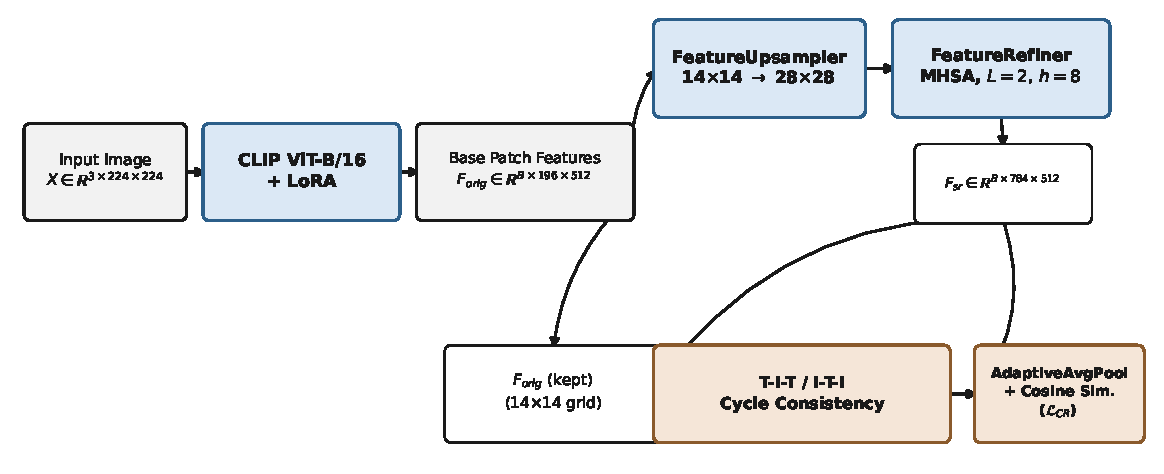
\includegraphics[width=0.92\textwidth]{figures/architecture.pdf}
\caption{FeatureSR pipeline. The frozen-text, LoRA-adapted CLIP backbone produces base patch features $F_{orig}$, which branch into (i) the FeatureUpsampler + FeatureRefiner path producing $F_{sr}$, used for the T-I-T/I-T-I cycle-consistency losses, and (ii) an unmodified copy of $F_{orig}$ used as the pooling target for the Cross-Resolution Consistency loss $\mathcal{L}_{CR}$.}
\label{fig:architecture}
\end{figure*}

\subsection{FeatureUpsampler}
Given the base patch feature sequence $\mathbf{F} \in \mathbb{R}^{B \times P \times d}$ ($P = 196, d = 512$):

\begin{enumerate}
\item \textbf{Spatial reshape}:
\[ \mathbf{F}_{\text{2D}} = \text{Reshape}(\mathbf{F}) \in \mathbb{R}^{B \times d \times H \times W} \quad (H=W=14) \]
\item \textbf{Bilinear spatial interpolation}:
\[ \mathbf{F}_{\text{interp}} = \text{Bilinear}(\mathbf{F}_{\text{2D}}, \text{scale}=2) \in \mathbb{R}^{B \times d \times 28 \times 28} \]
\item \textbf{Learnable residual correction}:
\[ \mathbf{R} = \text{Conv2D}_{3\times3}\big(\text{GELU}(\text{LN}(\text{Conv2D}_{3\times3}(\mathbf{F}_{\text{interp}})))\big) \]
\[ \mathbf{F}_{\text{up\_2D}} = \mathbf{F}_{\text{interp}} + \mathbf{R} \]
(Note: $\mathbf{R}$ is initialized near zero to preserve initial semantic structure.)
\item \textbf{Positional embedding injection}:
\[ \mathbf{F}_{\text{up}} = \text{Flatten}(\mathbf{F}_{\text{up\_2D}}) + \mathbf{P}_{\text{up}} \in \mathbb{R}^{B \times 784 \times 512} \]
where $\mathbf{P}_{\text{up}} \in \mathbb{R}^{1 \times 784 \times d}$ is a learnable positional embedding.
\end{enumerate}

\subsection{FeatureRefiner}
To capture long-range contextual spatial dependencies among the $N=784$ upsampled tokens, the sequence passes through $L=2$ Pre-LN Transformer blocks with multi-head self-attention ($h=8$ heads):

\[ \mathbf{X}^{(l)\prime} = \mathbf{X}^{(l-1)} + \text{MHSA}\big(\text{LN}_1(\mathbf{X}^{(l-1)})\big) \]
\[ \mathbf{X}^{(l)} = \mathbf{X}^{(l)\prime} + \text{MLP}\big(\text{LN}_2(\mathbf{X}^{(l)\prime})\big) \]

The output is normalized onto the unit hypersphere:
\[ \mathbf{F}_{\text{sr}} = \frac{\text{LN}_{\text{post}}(\mathbf{X}^{(L)})}{\|\text{LN}_{\text{post}}(\mathbf{X}^{(L)})\|_2} \in \mathbb{R}^{B \times 784 \times 512} \]

\section{Loss Functions and Objectives}

The total training objective is formulated as:
\[ \mathcal{L}_{\text{total}} = \mathcal{L}_{\text{CE}} + \lambda_1 \mathcal{L}_{\text{TIT}} + \lambda_2 \mathcal{L}_{\text{ITI}} + \lambda_3 \mathcal{L}_{\text{CR}} \]

\subsection{Cross-Resolution Consistency Loss ($\mathcal{L}_{\text{CR}}$)}
To prevent semantic distortion during upsampling, $\mathcal{L}_{\text{CR}}$ forces the pooled high-resolution representations to align with the un-upsampled base tokens:
\[ \mathbf{F}_{\text{pooled}} = \text{AdaptiveAvgPool2D}(\mathbf{F}_{\text{sr}}, (14,14)) \in \mathbb{R}^{B \times 196 \times d} \]
\[ \mathcal{L}_{\text{CR}} = 1 - \frac{1}{B P} \sum_{b=1}^{B}\sum_{p=1}^{P} \big\langle \hat{\mathbf{F}}_{\text{pooled}}^{(b,p)}, \hat{\mathbf{F}}_{\text{orig}}^{(b,p)} \big\rangle \]

\subsection{Vision--Language Cyclic Consistency ($\mathcal{L}_{\text{TIT}}, \mathcal{L}_{\text{ITI}}$)}
\begin{itemize}
\item $\mathcal{L}_{\text{TIT}}$: Text-to-Image-to-Text cyclic reconstruction matching class text embeddings with optimal $28\times28$ patch representations.
\item $\mathcal{L}_{\text{ITI}}$: Image-to-Text-to-Image cycle using Top-$k{=}10$ Semantic Anchors across data-augmented feature spaces.
\end{itemize}

\subsection{Domain-Adaptive Prompt Ensemble (Text-Side Enhancement)} \label{sec:promptensemble}

Orthogonal to FeatureSR's visual-side upsampling, a text-side enhancement module improves the anchor text embeddings $\mathbf{e}_i$ used throughout $\mathcal{L}_{\text{CE}}$, $\mathcal{L}_{\text{TIT}}$, and $\mathcal{L}_{\text{ITI}}$.

Given a raw class label $c_i$ and target domain $d$, a domain-specific semantic expansion function $\phi(c_i,d)$ maps abbreviated or terse labels into descriptive phrases (e.g., ISIC's \texttt{"MEL"} $\rightarrow$ \texttt{"melanoma, a malignant pigmented skin cancer lesion"}), and a domain-specific template bank $\mathcal{T}_d = \{t_1,\dots,t_M\}$ supplies $M$ paraphrastic prompt structures (e.g., \texttt{"a dermatoscopic photograph of \{c\}."}). The ensembled anchor embedding is the re-normalized mean of $M$ independently normalized template embeddings:

\begin{equation}
\resizebox{0.48\textwidth}{!}{$
\mathbf{e}_i = \dfrac{\dfrac{1}{M}\sum\limits_{m=1}^{M} \hat{g}_{\text{text}}\big(t_m(\phi(c_i,d))\big)}{\Big\|\dfrac{1}{M}\sum\limits_{m=1}^{M} \hat{g}_{\text{text}}\big(t_m(\phi(c_i,d))\big)\Big\|_2}, \quad \hat{g}_{\text{text}}(\cdot) = \dfrac{g_{\text{text}}(\cdot)}{\|g_{\text{text}}(\cdot)\|_2}
$}
\end{equation}

where $g_{\text{text}}(\cdot)$ is the frozen CLIP text encoder.

\subsection{The Train/Inference Consistency Requirement} \label{sec:consistency}

CLIP-LoRA~\cite{zanella2024cliplora} injects trainable low-rank parameters $\theta_{\text{LoRA}}$ (via LoRA~\cite{hu2022lora}) only into the attention projections of the visual tower (\S II-A--II-B); $g_{\text{text}}(\cdot)$ carries no trainable parameters at all. Consequently, $\theta_{\text{LoRA}}$ is optimized against whichever anchor-embedding function was in effect during training:

\begin{equation}
\resizebox{0.48\textwidth}{!}{$
\theta_{\text{LoRA}}^{*} = \arg\min_{\theta} \; \mathbb{E}\Big[\mathcal{L}_{\text{total}}\big(f_\theta(x),\; \mathbf{e}(c;\,\text{prompt}_{\text{train}})\big)\Big]
$}
\end{equation}

If inference substitutes a different anchor function, $\text{prompt}_{\text{infer}} \neq \text{prompt}_{\text{train}}$, the induced text-embedding distribution shifts relative to what $\theta_{\text{LoRA}}^{*}$ was calibrated against --- a covariate shift confined to the text branch, since the visual branch is unchanged. This is a \emph{post-hoc} application of \S\ref{sec:promptensemble} (ensemble enabled only at evaluation time) and was empirically found to be actively harmful: averaged over 4 target domains, post-hoc ensembling produced a $-7.81\%$ mean accuracy regression (5-way 5-shot), with ISIC 2018 collapsing by $-18.61\%$ --- the domain with the largest semantic-expansion magnitude in $\phi(\cdot,\cdot)$, consistent with the magnitude of the covariate shift being the driver of the regression.

The correction is to apply \S\ref{sec:promptensemble} identically during training and inference, i.e.\ compute $\mathbf{e}_i$ via the same $(\mathcal{T}_d,\phi)$ in both $\mathcal{L}_{\text{total}}$ and evaluation, so that $\theta_{\text{LoRA}}$ is calibrated to the distribution it will actually be evaluated against. This recovers the regression and, on 3 of 4 domains, yields a net improvement over the single-template baseline (\S\ref{sec:promptresults}).

\section{Optimization and Empirical Results}

\subsection{Optimization Protocol}
\begin{itemize}
\item \textbf{Optimizer}: Adam (\texttt{weight\_decay=5e-4})
\item \textbf{Peak learning rate}: \texttt{lr = 3e-5}
\item \textbf{Warmup schedule}: 5 epochs linear warmup followed by cosine annealing decay down to \texttt{1e-6} over 100 epochs.
\end{itemize}

\subsection{Benchmark Verification (Strict Few-Shot)}

\begin{table}[t]
\centering
\caption{Feature-SR vs.\ baseline, 5-way 5-shot (400 episodes).}
\label{tab:fsr5shot}
\footnotesize
\setlength{\tabcolsep}{3.5pt}
\begin{tabular}{lcccc}
\toprule
Dataset & Base. (14$^2$) & F-SR (28$^2$) & $\Delta$ & Peak \\
\midrule
EuroSAT       & $88.79{\pm}0.48\%$ & $\mathbf{90.16{\pm}0.40\%}$ & $\mathbf{+1.37\%}$ & 90.43\% \\
CropDiseases  & $89.68{\pm}0.70\%$ & $\mathbf{90.61{\pm}0.65\%}$ & $\mathbf{+0.93\%}$ & 90.41\% \\
ISIC 2018     & $41.44{\pm}0.64\%$ & $\mathbf{43.20{\pm}0.63\%}$ & $\mathbf{+1.76\%}$ & 43.30\% \\
ChestX        & $22.43{\pm}0.46\%$ & $\mathbf{22.46{\pm}0.42\%}$ & $\mathbf{+0.03\%}$ & 22.64\% \\
\midrule
\textbf{Average} & \textbf{60.59\%} & \textbf{61.61\%} & \textbf{+1.02\%} & --- \\
\bottomrule
\end{tabular}
\end{table}

\begin{table}[t]
\centering
\caption{Feature-SR vs.\ baseline, 5-way 1-shot (100 episodes).}
\label{tab:fsr1shot}
\footnotesize
\setlength{\tabcolsep}{3.5pt}
\begin{tabular}{lcccc}
\toprule
Dataset & Base. (14$^2$) & F-SR (28$^2$) & $\Delta$ & Peak \\
\midrule
EuroSAT       & $\mathbf{80.59{\pm}1.29\%}$ & $80.29{\pm}1.54\%$ & $-0.30\%$ & 82.00\% \\
CropDiseases  & $\mathbf{77.77{\pm}2.00\%}$ & $76.37{\pm}2.22\%$ & $-1.40\%$ & 80.00\% \\
ISIC 2018     & $30.93{\pm}1.11\%$ & $\mathbf{32.63{\pm}1.20\%}$ & $\mathbf{+1.70\%}$ & 32.91\% \\
ChestX        & $\mathbf{21.95{\pm}0.86\%}$ & $21.51{\pm}0.88\%$ & $-0.44\%$ & 21.33\% \\
\midrule
\textbf{Average} & \textbf{52.81\%} & \textbf{52.70\%} & $-0.11\%$ & --- \\
\bottomrule
\end{tabular}
\end{table}

\subsection{Prompt Ensemble: Post-hoc Regression vs.\ Train/Inference-Consistent Fix} \label{sec:promptresults}

\begin{table}[t]
\centering
\caption{Post-hoc vs.\ train/inference-consistent Prompt Ensemble, 5-way 5-shot (400 episodes). ``Post-hoc'' = $\text{prompt}_{\text{infer}} \neq \text{prompt}_{\text{train}}$; ``Consistent'' = $\text{prompt}_{\text{infer}} = \text{prompt}_{\text{train}}$.}
\label{tab:promptensemble}
\scriptsize
\setlength{\tabcolsep}{3pt}
\begin{tabular}{lccc}
\toprule
Dataset & Baseline & Post-hoc & Consistent \\
\midrule
EuroSAT      & $90.17{\pm}0.89\%$ & $84.15\%(-6.03\%)$  & $\mathbf{93.81{\pm}0.32\%}(+3.64\%)$ \\
CropDiseases & $90.03{\pm}1.36\%$ & $85.04\%(-4.99\%)$  & $\mathbf{90.57{\pm}0.64\%}(+0.54\%)$ \\
ISIC 2018    & $43.76{\pm}1.38\%$ & $25.15\%(-18.61\%)$ & $\mathbf{44.49{\pm}0.61\%}(+0.73\%)$ \\
ChestX       & $22.88{\pm}0.83\%$ & $21.28\%(-1.60\%)$  & $22.79{\pm}0.45\%(-0.09\%)$ \\
\midrule
\textbf{Average} & \textbf{61.71\%} & $53.90\%(-7.81\%)$ & \textbf{62.92\%}$(+1.21\%)$ \\
\bottomrule
\end{tabular}
\end{table}

\noindent\textit{Note: the baseline in this table is drawn from an independent training run relative to Tables~\ref{tab:fsr5shot}--\ref{tab:fsr1shot} ($61.71\%$ vs.\ $60.59\%$ average); the two baselines are not the same checkpoint and should not be compared in absolute terms --- only $\Delta$ within a matched training run is meaningful.}

\subsection{Combined Feature-SR + Prompt Ensemble} \label{sec:combined}

Both modules were enabled jointly during training (identical prompt used at train- and inference-time, per \S\ref{sec:consistency}) to test whether the visual-side and text-side gains compose (5-way 5-shot, 400 episodes):

\begin{table}[t]
\centering
\caption{Combined Feature-SR + Prompt Ensemble results, 5-way 5-shot (400 episodes).}
\label{tab:combined}
\footnotesize
\setlength{\tabcolsep}{3.5pt}
\begin{tabular}{lccccc}
\toprule
Dataset & Base. & Ens.-only & \textbf{FSR+Ens.} & $\Delta$ & Epoch \\
\midrule
EuroSAT      & 90.17\% & 93.81\% & $\mathbf{94.54{\pm}0.30\%}$ & $\mathbf{+4.37\%}$ & 40 \\
CropDiseases & 90.03\% & 90.57\% & $\mathbf{90.97{\pm}0.60\%}$ & $\mathbf{+0.94\%}$ & 50 \\
ISIC 2018    & 43.76\% & 44.49\% & $\mathbf{44.77{\pm}0.65\%}$ & $\mathbf{+1.01\%}$ & 40 \\
ChestX       & 22.88\% & 22.79\% & $\mathbf{22.96{\pm}0.47\%}$ & $+0.08\%$ & 70 \\
\midrule
\textbf{Average} & \textbf{61.71\%} & \textbf{62.92\%} & \textbf{63.31\%} & \textbf{+1.60\%} & --- \\
\bottomrule
\end{tabular}
\end{table}

All 4/4 domains satisfy $\text{Baseline} < \text{Ensemble-only} < \text{Feature-SR+Ensemble}$, i.e.\ a strictly monotonic stack with no negative interaction term observed, consistent with the two mechanisms acting on disjoint parameter/embedding spaces (visual-side LoRA + FeatureUpsampler/Refiner vs.\ text-side anchor embeddings). A secondary effect was observed on ISIC 2018: the ensemble-only run overfits sharply past epoch 10 (peak $44.44\% \rightarrow 38.38\%$ by epoch 100), whereas the combined run remains stable in the $43$--$45\%$ band through epoch 100 (best epoch 40), suggesting $\mathcal{L}_{\text{CR}}$ (\S III-A) contributes an incidental regularizing effect under extreme few-shot sample sizes ($n=35$).

\section{Computational Complexity}

\begin{table}[t]
\centering
\caption{Parameter and memory overhead by component.}
\label{tab:complexity}
\small
\begin{tabular}{lcc}
\toprule
Component & Trainable Params & GPU Mem. \\
\midrule
CLIP-LoRA Backbone & 0.22\,M & $\sim$0.44\,MB \\
FeatureUpsampler & 2.36\,M & $\sim$4.7\,MB \\
FeatureRefiner (2 blocks) & 7.99\,M & $\sim$15.9\,MB \\
\textbf{Total added by FeatureSR} & \textbf{10.35\,M} & \textbf{$\sim$21\,MB} \\
Prompt Ensemble & 0\,M (frozen) & Negligible \\
\bottomrule
\end{tabular}
\end{table}

Total VRAM including the frozen CLIP-LoRA backbone is $\sim$2.4\,GB. The Prompt Ensemble row incurs $M\times$ text-encoder forward passes under \texttt{torch.no\_grad()}, with no backward pass.

\section{Known Limitations} \label{sec:limitations}

\subsection{ChestX: A Backbone-Architecture Ceiling, Not a Method Failure}

Across every experiment in this document, ChestX consistently shows the smallest gain from either enhancement (Feature-SR: $+0.03\%$; Prompt Ensemble: $-0.09\%$; combined: $+0.08\%$). Cross-referencing the CC-CDFSL paper's~\cite{zhao2026ccdfsl} own Appendix Table 9 (comparison against SOTA CDFSL methods, 5-way 5-shot) shows this is not specific to FeatureSR or the prompt module:

\begin{table}[t]
\centering
\caption{ChestX 5-way 5-shot comparison with SOTA CDFSL methods (source: CC-CDFSL paper Appendix Table 9).}
\label{tab:chestx-sota}
\small
\begin{tabular}{lcc}
\toprule
Method & Backbone & ChestX \\
\midrule
IM-DCL~\cite{xu2024imdcl} (TIP-24) & ResNet10 & $\mathbf{28.93\%}$ \\
DAMIM-FT~\cite{ma2025damim} (AAAI-25) & ViT/DINO & 27.82\% \\
AttnTemp~\cite{zou2024attntemp} (NeurIPS-24) & ViT/DINO & 27.72\% \\
CLIP-LoRA + CC-CDFSL~\cite{zhao2026ccdfsl} & ViT/CLIP & 25.47\% \\
CLIP-LoRA~\cite{zanella2024cliplora} (baseline) & ViT/CLIP & 24.44\% \\
\bottomrule
\end{tabular}
\end{table}

Every ViT/CLIP-based method in the comparison --- including the CC-CDFSL paper's own full method --- underperforms ResNet-based competitors on ChestX specifically. This suggests the limiting factor on ChestX is the ViT/CLIP backbone's inductive bias relative to the fine-grained, low-contrast local textures characteristic of grayscale radiographs, a ceiling that sits upstream of both FeatureSR (which upsamples this same backbone's patch grid) and the text-side prompt module. Closing this gap would require backbone-level changes and is out of scope for this document.

\begin{thebibliography}{99}

\bibitem{zhao2026ccdfsl} Y. Zhao, Y. Zou, Y. Li, and R. Li, ``Interpretable cross-domain few-shot learning with rectified target-domain local alignment,'' in \emph{Proc. IEEE/CVF Conf. Computer Vision and Pattern Recognition (CVPR)}, 2026.

\bibitem{radford2021clip} A. Radford, J. W. Kim, C. Hallacy, A. Ramesh, G. Goh, S. Agarwal, G. Sastry, A. Askell, P. Mishkin, J. Clark, G. Krueger, and I. Sutskever, ``Learning transferable visual models from natural language supervision,'' in \emph{Proc. Int. Conf. Machine Learning (ICML)}, 2021, pp. 8748--8763.

\bibitem{zanella2024cliplora} M. Zanella and I. Ben Ayed, ``Low-rank few-shot adaptation of vision-language models,'' in \emph{Proc. IEEE/CVF Conf. Computer Vision and Pattern Recognition Workshops (CVPRW)}, 2024, pp. 1593--1603.

\bibitem{hu2022lora} E. J. Hu, Y. Shen, P. Wallis, Z. Allen-Zhu, Y. Li, S. Wang, L. Wang, and W. Chen, ``LoRA: Low-rank adaptation of large language models,'' in \emph{Proc. Int. Conf. Learning Representations (ICLR)}, 2022.

\bibitem{guo2020bscdfsl} Y. Guo, N. C. Codella, L. Karlinsky, J. V. Codella, J. R. Smith, K. Saenko, T. Rosing, and R. Feris, ``A broader study of cross-domain few-shot learning,'' in \emph{Proc. European Conf. Computer Vision (ECCV)}, 2020, pp. 124--141.

\bibitem{helber2019eurosat} P. Helber, B. Bischke, A. Dengel, and D. Borth, ``EuroSAT: A novel dataset and deep learning benchmark for land use and land cover classification,'' \emph{IEEE J. Sel. Topics Appl. Earth Observ. Remote Sens.}, pp. 2217--2226, 2019.

\bibitem{mohanty2016plantdisease} S. P. Mohanty, D. P. Hughes, and M. Salath\'e, ``Using deep learning for image-based plant disease detection,'' \emph{Frontiers in Plant Science}, 2016.

\bibitem{codella2019isic} N. Codella, V. Rotemberg, P. Tschandl, M. E. Celebi, S. Dusza, D. Gutman, B. Helba, A. Kalloo, K. Liopyris, M. Marchetti, \emph{et al.}, ``Skin lesion analysis toward melanoma detection 2018: A challenge hosted by the International Skin Imaging Collaboration (ISIC),'' \emph{arXiv preprint arXiv:1902.03368}, 2019.

\bibitem{wang2017chestxray8} X. Wang, Y. Peng, L. Lu, Z. Lu, M. Bagheri, and R. M. Summers, ``ChestX-ray8: Hospital-scale chest X-ray database and benchmarks on weakly-supervised classification and localization of common thorax diseases,'' in \emph{Proc. IEEE Conf. Computer Vision and Pattern Recognition (CVPR)}, 2017, pp. 2097--2106.

\bibitem{wang2021realesrgan} X. Wang, L. Xie, C. Dong, and Y. Shan, ``Real-ESRGAN: Training real-world blind super-resolution with pure synthetic data,'' in \emph{Proc. IEEE/CVF Int. Conf. Computer Vision Workshops (ICCVW)}, 2021, pp. 1905--1914.

\bibitem{ma2025damim} R. Ma, Y. Zou, Y. Li, and R. Li, ``Reconstruction target matters in masked image modeling for cross-domain few-shot learning,'' in \emph{Proc. AAAI Conf. Artificial Intelligence}, 2025, pp. 19305--19313.

\bibitem{xu2024imdcl} H. Xu, L. Liu, S. Zhi, S. Fu, Z. Su, M.-M. Cheng, and Y. Liu, ``Enhancing information maximization with distance-aware contrastive learning for source-free cross-domain few-shot learning,'' \emph{IEEE Trans. Image Process.}, pp. 2058--2073, 2024.

\bibitem{zou2024attntemp} Y. Zou, R. Ma, Y. Li, and R. Li, ``Attention temperature matters in ViT-based cross-domain few-shot learning,'' in \emph{Proc. Conf. Neural Information Processing Systems (NeurIPS)}, 2024.

\end{thebibliography}

\end{document}
